\begin{table}[t]
\caption{Emission saving vs.\ FCFS (\%) / harm rate (\% of shifted jobs emitting more than at submission) at 70\% utilisation, $S{=}12$\,h, mean of 10 weekly offsets. GB-op uses NESO's own forecasts.}
\label{tab:main}
\centering\scriptsize\setlength{\tabcolsep}{2.2pt}
\begin{tabular}{lrrrrrrr}
\toprule
Region & P3 & P4 & P4-$\lambda$ & P7 & P8 & P9-r & CG \\
\midrule
GB-op$^\dagger$ & 7.8/37 & 2.8/17 & 6.9/28 & 6.1/23 & 7.9/26 & 7.7/35 & 8.7/32 \\
GB-25 & 7.5/36 & 0.6/13 & 3.7/24 & 2.7/22 & 6.2/28 & 7.4/33 & 9.6/27 \\
CISO & 4.1/34 & 2.9/26 & 4.3/33 & 4.2/31 & 4.2/24 & 4.1/33 & 4.5/32 \\
ERCO & 4.5/30 & 0.1/16 & 2.4/25 & 2.2/21 & 4.0/23 & 4.4/28 & 5.4/27 \\
PJM & 0.9/38 & 0.1/25 & 0.4/36 & 0.4/33 & 0.5/36 & 0.8/37 & 1.3/27 \\
MISO & 1.8/35 & 0.1/31 & 0.4/29 & 0.9/26 & 1.4/31 & 1.6/35 & 2.8/29 \\
\midrule
Mean & 4.4/35 & 1.1/21 & 3.0/29 & 2.8/26 & 4.0/28 & 4.3/33 & 5.4/29 \\
\bottomrule
\end{tabular}
\end{table}

\begin{table}[t]
\caption{Utilisation sweep (mean of six regions, $S{=}12$\,h): harm rate (\%) and saving (\%). Even clairvoyant greedy's harm rises with load; all of it is contention (its voluntary harm is 0).}
\label{tab:util}
\centering\scriptsize\setlength{\tabcolsep}{2.6pt}
\begin{tabular}{lrrrrrr}
\toprule
 & \multicolumn{2}{c}{50\%} & \multicolumn{2}{c}{70\%} & \multicolumn{2}{c}{90\%} \\
\cmidrule(lr){2-3}\cmidrule(lr){4-5}\cmidrule(lr){6-7}
Policy & Harm & Sav. & Harm & Sav. & Harm & Sav. \\
\midrule
Clairvoyant greedy (CG) & 13 & 7.5 & 29 & 5.4 & 41 & 2.4 \\
Point P2 & 27 & 5.6 & 37 & 4.1 & 44 & 2.0 \\
Point+replan P3 & 26 & 5.8 & 35 & 4.4 & 43 & 2.3 \\
Conformal UB P4 & 11 & 1.3 & 21 & 1.1 & 46 & 0.6 \\
Decision-conf.\ P7 & 14 & 3.3 & 26 & 2.8 & 43 & 1.7 \\
Headroom P8 & 21 & 5.6 & 28 & 4.0 & 41 & 1.8 \\
Jitter P9-r & 22 & 5.6 & 33 & 4.3 & 43 & 2.2 \\
\midrule
P3 p95 slowdown & 5.8 &  & 6.8 &  & 34.2 &  \\
P3 non-defer.\ wait (min) & 0.6 &  & 3.8 &  & 62.8 &  \\
\bottomrule
\end{tabular}
\end{table}


\section{Measurement: When Does Deferral Backfire?}\label{sec:measure}

\textbf{Harm is common, even with perfect foresight.}
Table~\ref{tab:main} reports savings and harm at 70\% utilisation. On GB-op, where every forecast
error comes from NESO's published forecasts, point-forecast greedy with re-planning (P3) saves
\res{V2U}{GBop-S12-utiltarget0.7}{P3}{savingpct}\% of emissions but harms
\res{V2U}{GBop-S12-utiltarget0.7}{P3}{harmrate}\% of the jobs it shifts. Clairvoyant greedy (CG) saves
\res{V2U}{GBop-S12-utiltarget0.7}{P5}{savingpct}\% and still harms
\res{V2U}{GBop-S12-utiltarget0.7}{P5}{harmrate}\%. Across the six regions the pattern holds
(means \res{V2U}{ALL-S12-utiltarget0.7}{P3}{harmrate}\% and
\res{V2U}{ALL-S12-utiltarget0.7}{P5}{harmrate}\%). CG never harms a job that could have started
at submission: its \emph{voluntary} harm is \res{V2U}{ALL-S12-utiltarget0.7}{P5}{harmratevoluntary}\%
by construction. Every one of its harmed jobs arrived to a cluster whose free capacity had already
been reserved, mostly by other deferred jobs.

\textbf{Harm grows with load (Table~\ref{tab:util}, Fig.~\ref{fig:util}).}
Holding the workload fixed and scaling capacity, CG's harm rate rises from
\res{V2U}{ALL-S12-utiltarget0.5}{P5}{harmrate}\% at 50\% utilisation to
\res{V2U}{ALL-S12-utiltarget0.7}{P5}{harmrate}\% at 70\% and
\res{V2U}{ALL-S12-utiltarget0.9}{P5}{harmrate}\% at 90\%, while its saving falls from
\res{V2U}{ALL-S12-utiltarget0.5}{P5}{savingpct}\% to \res{V2U}{ALL-S12-utiltarget0.9}{P5}{savingpct}\%.
The same holds for every policy. Mean waiting time of \emph{non-deferrable} jobs under P3 grows from
\res{V2U}{ALL-S12-utiltarget0.5}{P3}{waitminmeannondeferrable} to
\res{V2U}{ALL-S12-utiltarget0.9}{P3}{waitminmeannondeferrable} minutes, against
\res{V2U}{ALL-S12-utiltarget0.9}{P0}{waitminmeannondeferrable} under carbon-agnostic FCFS at 90\%.
Deferred reservations crowd out work that cannot wait. Longer slack has the same effect: in the
65\%-utilisation grid CG harms \res{V1S}{ALL-S2}{P5}{harmrate}\% of shifted jobs at 2\,h slack
and \res{V1S}{ALL-S12}{P5}{harmrate}\% at 12\,h, as more jobs can reach the same trough.
A slow ramp would suggest that CI simply mean-reverts within the slack window. Instead the growth is
steep and monotone in load, with zero voluntary CG harm, so the mechanism is contention.
A joint offline optimum would schedule around this contention, so our figures bound the harm
attributable to greedy deferral rather than the minimum cost of shifting per se.

\begin{figure}[t]
\centering
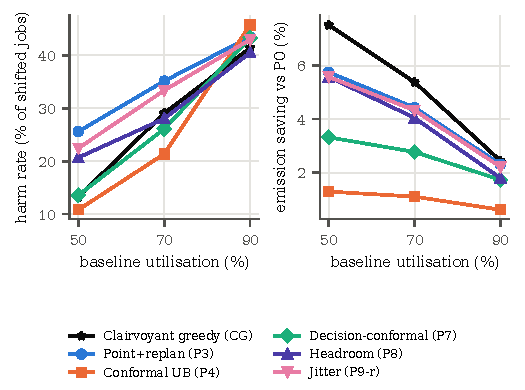
\includegraphics[width=\columnwidth]{figs/fig_util.pdf}
\caption{Harm rate and saving vs.\ baseline utilisation (mean of six regions, $S{=}12$\,h). Clairvoyant-greedy harm
rises with load: congestion, not forecast error.}
\label{fig:util}
\end{figure}

\textbf{Attribution (Fig.~\ref{fig:decomp}).}
Eq.~\eqref{eq:decomp} splits each harmed job's excess exactly. For single-decision policies the
re-planning term is zero and the split is unambiguous. For point-forecast greedy (P2), forecast error
accounts for \res{V2U}{POOL-S12-utiltarget0.5}{P2}{shareforecast}\% of harmful excess at 50\%
utilisation, but only \res{V2U}{POOL-S12-utiltarget0.7}{P2}{shareforecast}\% at 70\% and
\res{V2U}{POOL-S12-utiltarget0.9}{P2}{shareforecast}\% at 90\%. The remainder is contention: the job
did not run in the slot its rule wanted. CG's forecast term is negative
(\res{V2U}{POOL-S12-utiltarget0.7}{P5}{shareforecast}\% at 70\%), since the slots it wanted were
genuinely cleaner; all of its harm is contention. Forecast error is therefore a first-order cause
only in a lightly loaded cluster. For policies that re-plan hourly the re-planning term also absorbs
displacement by capacity, so we report their attribution only in aggregate.

\begin{figure}[t]
\centering
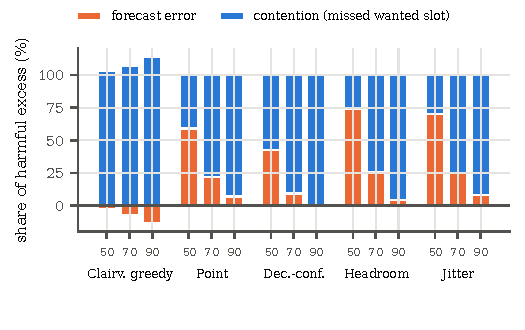
\includegraphics[width=\columnwidth]{figs/fig_decomp.pdf}
\caption{Where harmful excess comes from (single-decision policies, all regions pooled; 50/70/90\% utilisation).
Forecast error dominates only at low load; contention dominates otherwise.}
\label{fig:decomp}
\end{figure}
